% ### Uses XeLaTeX ### %
% ### Needs beamer-master ### %
\documentclass[aspectratio=169]{beamer} %. Aspect Ratio 16:9
\usepackage{textgreek}
\usetheme{AI2} % beamerthemeSprace.sty
% DATA FOR FOOTER
\date{2019}
\title{}
\author{}
\institute{Advanced Institute for Artificial Intelligence (AI2)}
\begin{document}    
% ####################################
% FIRST SLIDE 						:: \SliTit{<Title of the Talk>}{<Author Name>}{<Intitution>}
% SLIDE SUB-TITLE					:: \SliSubTit{<Title of the Chapter>}{<Title of the Section>}
% SLIDE WITH TITLE 					:: \SliT{<Title>}{Content}
% SLIDE NO TITLE 						:: \Sli{<Content>} 
% SLIDE DOUBLE COLUMN WITH TITLE 	:: \SliDT{<Title>}{<First Column>}{<Second Column>}
% SLIDE DOUBLE COLUMN NO TITLE 		:: \SliD{<First Column>}{<Second Column>}
% SLIDE ADVANCED WITH TITLE 			:: \SliAdvT{<Title>}{<Content>}
% SLIDE ADVANCED  NO TITLE 			:: \SliAdv{<Content>}
% SLIDE ADVANCED DOUBLE TITLE 		:: SliAdvDT{<Title>}{<First Column>}{<Second Column>}
% SLIDE ADVANCED DOUBLE NO TITLE 	:: SliAdvD{<First Column>}{<Second Column>}
% ITEMIZE 							:: \begin{itemize}  \IteOne{1st Level} \IteTwo {2nd Level} \IteThr{3rd Level} \end{itemize}
% SECTION 							:: \secx{Section} | \secxx{Sub-Section}
% COLOR BOX 						:: \blu{blue} + \red{red} + \yel{yellow} + \gre{green}
% FRAME 							:: \fra{sprace} \frab{blue} \frar{red} + \fray{yellow} + \frag{green}	
% REFERENCE						:: \refer{<doi number>}
% FIGURE 							::  \img{X}{Y}{<scale>}{Figures/.png} 
% FIGURE							:: \begin{center}\includegraphics[scale=<#>]{Figures/.png}\end{center}
% PROJECT STATUS					:: \planned\~    \started\~   \underway\~   \done\~   
% EXERCICIO							:: \Exe{<#>}{<text>}
% STACKREL							:: \underset{<down>}{<up>}
% FLUSH LEFT						:: \begin{flalign*}  & <1st equation> & \\  & <12nd equation>  & \\ \end{flalign*}
% REAL / IMAGINAY					:: \Re / \Im
% SLASH								:: \sl{} or \sl
% BOLD MATH							:: \pmb{<>}
% ####################################
%
% FIRST SLIDE :: DO NOT BREAK LINE !!!
\SliTit{Aprendizagem de Máquina}{Advanced Institute for Artificial Intelligence}{https://advancedinstitute.ai}

\SliT{Estatística}{

Agenda
\begin{itemize}
\IteOne{Bibliotecas}
\IteOne{Análise Estatística Descritiva}
\IteTwo{Tendência central}
\IteTwo{Dispersão}
\IteTwo{Interpretação}
\IteOne{Correlação}
\IteOne{Análise de probabilidades}
\end{itemize}

}
\SliT{Estatística}{

Bibliotecas Python para Estatística
\begin{itemize}
\IteOne{Scikit-Learn}
\IteTwo{Provê suporte a utilização de algoritmos de aprendizagem de máquina}
\IteOne{Scipy Stats}
\IteTwo{Função estatísticas elementares}
\IteOne{MatplotLib}
\IteTwo{Biblioteca para montar gráficos}
\IteOne{Pandas e Numpy}
\IteTwo{Algumas funções estatístiticas e de gráficos estão embutidas nessas bibliotecas}
\end{itemize}

}

% SLIDE WITH TITLE
\SliT{Estatística}{
Análise Estatística
\begin{itemize}
\IteOne{Passo fundamental para utilização de técnicas de aprendizagem de máquina}
\IteTwo{Aprofundar o entendimento quanto aos dados disponíveis}
\IteTwo{Preparação adequada dos dados}
\IteTwo{Ex: Dados faltantes}
\IteTwo{Ex: Outliers}
\IteTwo{Ex: Segmentação adequada}
\end{itemize}

}

\SliT{Estatística}{

Descrição de Dados

\begin{itemize}
\IteOne{Dados organizados em tabelas dificultam análises }
\IteOne{Gráficos são essenciais para realização de análises de modo mais prático}
\IteOne{Medidas de tendência central e variabilidade complementam tais análises e facilitam comparações}
\end{itemize}

}

\SliT{Estatística}{

Tipos de Dados e Gráficos

\begin{itemize}
\IteOne{Dados Qualitativos}
\IteTwo{Gráfico de barra}
\IteTwo{Gráfico de pizza}
\IteOne{Dados Quantitativos}
\IteTwo{Histograma}
\IteTwo{Box}
\IteTwo{Área}
\IteTwo{Linha}
\IteTwo{Scatter}
\end{itemize}

}

\SliT{Estatística}{

Estimativa de densidade por Kernel (KDE - Kernel Density Estimate)

\begin{itemize}
\IteOne{forma não-paramétrica para estimar a Função densidade de probabilidade de uma variável aleatória.}
\IteOne{Possui a propriedade de estimar de forma continua de acordo com um kernel adequado (curva normal por exemplo)}
\IteOne{Opção de visualização a histogramas}

\end{itemize}

}

\SliT{Estatística}{

Tendência central

\begin{itemize}
\IteOne{Média ($\mu$): soma dos valores dividido pela quantidade de dados}
\IteOne{Mediana: valor situado no meio da amostra, quando a amostra está ordenada}
\IteOne{Moda: valor mais frequente na amostra}
\end{itemize}


}

\SliT{Estatística}{

Dispersão

\begin{itemize}
\IteOne{Desvio médio: módulo da média aritmética dos desvios de cada elemento da série para a média da série}
\IteOne{Variância: mesmo conceito do desvio médio trocando módulo por elevar a diferença ao quadrado}
\IteOne{Desvio Padrão ($\sigma$): é representado como a raiz quadrada da variância}

\end{itemize}

}

\SliT{Estatística}{

Interpretação da Dispersão
\begin{itemize}
\IteOne{Quanto mais uniforme forem os valores, mais próximo de zero estará o desvio padrão.}

\IteOne{Quando todos valores são iguais o desvio padrão é zero. Assim a amostra é perfeitamente uniforme.}

\IteOne{Quando estamos interessados em saber qual conjunto de valores possui uma maior regularidade podemos usar tanto a variância, como o desvio padrão.}

\IteOne{O desvio padrão é expresso na mesma unidade de medida das variáveis do conjunto.}

\end{itemize}
}

\SliT{Estatística}{

Variância: 

\begin{itemize}
\IteOne{Variância simples: soma do desvio quadrado de cada valor em relação a média dividido por n-1 (população -1)}
\IteOne{Desvio padrão simples: raiz quadrada da variância simples}
\end{itemize}

\begin{itemize}
\IteOne{Quando utilizamos a população completa é comum utilizar a população -1 para ajuste estatístico}
\end{itemize}
}

%\SliT{Estatística}{
%

%\begin{itemize}
%\IteTwo{média da amostra: $\overline{x}$ }
%\IteTwo{média da população: $\overline{\mu}$ }

%\IteOne{$s^{2}$ variancia amostral}
%\IteOne{$s$ desvio padrão amostral}
%\IteOne{$\mu^{2}$ variancia da população}
%\IteOne{$\mu$ desvio padrão da população}
%\end{itemize}

%}
\SliT{Estatística}{

Distribuição Normal
\begin{itemize}
\IteOne{É uma mais importantes distribuições de probabilidade que caracteriza muitos fenômenos aleatórios}
\IteTwo{Fenômenos naturais}
\IteTwo{Altura}
\IteTwo{pressão sangüínea}
\IteOne{Desempenham papel importante nos métodos de inferência estatística}
\IteOne{A distribuição é normal é uma variável aleatória contínua tem uma distribuição  em forma de sino.}
%\IteOne{É determinada pela média (μ) e desvio padrão (σ)}
\end{itemize}

}

\SliT{Estatística}{

Distribuições Normais com diferentes valores de média e desvio padrão

\begin{center}
    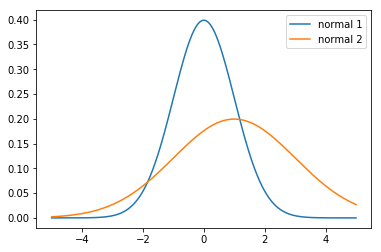
\includegraphics[scale=0.60]{nc2.png}     
    \end{center}
}

\SliT{Estatística}{

Distribuições paramétricas 

\begin{itemize}
\IteOne{regra empírica : define a probabilidade dos valores estarem em intervalos definidos pela média e desvio padrão}
\IteTwo{$\mu$ + $\sigma$ e $\mu$ - $\sigma$: 68\% }
\IteTwo{$\mu$ + 2*$\sigma$ e $\mu$ - 2*$\sigma$: 95\%}
\IteTwo{$\mu$ + 3*$\sigma$ e $\mu$ - 3*$\sigma$: 99\% }
\IteOne{z-score: representa a distância entre uma dada medida e a média em termos de desvio padrão}
\end{itemize}

}

\SliT{Estatística}{

\begin{center}
    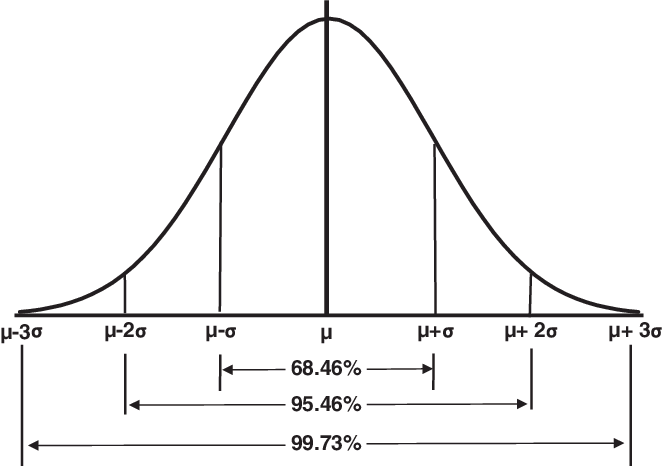
\includegraphics[scale=0.35]{nc1.png}     
    \end{center}
}


%\SliT{Estatística}{

%Distorção da Distribuição
%\begin{itemize}
%\IteOne{Quando média é maior que mediana é uma distribuição distorcida (\textit{skewed}) para direita}
%\IteOne{Quando média é menor que mediana é uma distribuição distorcida (\textit{skewed}) para esquerda}
%\IteOne{Quando média é próxima da mediana a distribuição é  simétrica}
%\end{itemize}
%}


% SLIDE WITH TITLE
\SliT{Estatística}{

\begin{itemize}
\IteOne{Covariância é uma medida sada para comparar o comportamento de duas ou mais variáveis}
\IteTwo{Mede como duas ou mais variáveis variam em conjunto de suas médias}
\IteOne{É possível identificar se diferentes variáveis possuem algum padrão comum entre si. }
\end{itemize}
}

\SliT{Estatística}{

\begin{itemize}

\IteOne{Por exemplo, uma variável que mede acidentes por dia em uma região e outra variável que mede velocidade média nessa mesma região.}

\IteOne{Tais padrões comuns permitem tomar conclusões a respeito da base em estudo }
\IteOne{Importante destacar que correlação não implica causalidade obrigatoriamente}

\end{itemize}
}

% SLIDE WITH TITLE
\SliT{Estatística}{

Correlação
\begin{itemize}
\IteOne{Utiliza-se a covariância e o desvio padrão como base para definir métricas de correlação}

\IteTwo{ A correlação perto de -1 é uma anti-correlação perfeita }
\IteTwo{ A correlação perto de 0 indica que não há correlação }
\IteTwo{ A correlação perto de 1 é uma correlação perfeita }

\end{itemize}

}

\end{document}